% Report for 204341 final assignment. Build: latexmk -pdf main.tex (see docs/workflow.md).
% Page rule: 10-15 pages without the cover page; 12 pt Times New Roman; A4.
% Generated files: references.bib and generated/*.tex come from scripts/make_report_data.py. Do not edit them.
\documentclass[12pt,a4paper]{article}

\usepackage{iftex}
\ifPDFTeX
  \usepackage[T1]{fontenc}
  \usepackage{newtxtext}% Times-like fallback; use XeLaTeX or LuaLaTeX for Times New Roman itself
\else
  \usepackage{fontspec}
  \IfFontExistsTF{Times New Roman}{\setmainfont{Times New Roman}}{\setmainfont{TeX Gyre Termes}}
  % Times New Roman has no Thai glyphs. Some prompts in the appendix are in Thai, so \thai{...} switches font.
  \IfFontExistsTF{Noto Sans Thai}{\newfontfamily\thaifont{Noto Sans Thai}}{%
    \IfFontExistsTF{Tahoma}{\newfontfamily\thaifont{Tahoma}}{%
      \IfFontExistsTF{Leelawadee UI}{\newfontfamily\thaifont{Leelawadee UI}}{\newfontfamily\thaifont{Loma}}}}
\fi
\ifPDFTeX
  \newcommand{\thai}[1]{#1}
\else
  \newcommand{\thai}[1]{{\thaifont\XeTeXlinebreaklocale "th"\XeTeXlinebreakskip=0pt plus 1pt #1}}
\fi
\usepackage[a4paper,margin=2cm]{geometry}
\usepackage{array}
\usepackage{longtable}
\usepackage{graphicx}
\usepackage{cite}% sort and compress citation numbers such as [1, 2, 4]
\renewcommand{\topfraction}{0.9}% let the 0.66-page figure float to the top of a page
\renewcommand{\textfraction}{0.1}
\usepackage[hidelinks]{hyperref}
\makeatletter\g@addto@macro\UrlBreaks{\do\-}\makeatother% allow a line break after a hyphen in a long URL
\makeatletter% tighter heading spacing: font size stays 12 pt
\renewcommand\section{\@startsection{section}{1}{\z@}{2.6ex \@plus .6ex \@minus .2ex}{1.2ex \@plus .2ex}{\normalfont\large\bfseries}}
\renewcommand\paragraph{\@startsection{paragraph}{4}{\z@}{1.6ex \@plus .6ex \@minus .2ex}{-1em}{\normalfont\normalsize\bfseries}}
\makeatother
\newenvironment{promptlist}{\begin{list}{}{\setlength{\leftmargin}{0em}\setlength{\itemsep}{3pt}\setlength{\topsep}{1pt}\setlength{\parsep}{0pt}\setlength{\labelwidth}{0em}}}{\end{list}}

\setlength{\emergencystretch}{1.5em}
\linespread{0.96}% about the leading of single spacing in Word for 12 pt Times New Roman
% Generated by scripts/make_report_data.py from knowledge-base/ and prompts/. Do not edit by hand.
\newcommand{\logsTotal}{83}
\newcommand{\logsSignificant}{4}
\newcommand{\claimsTotal}{521}
\newcommand{\claimsHumanVerified}{372}
\newcommand{\claimsAiChecked}{132}
\newcommand{\claimsAssumption}{17}
\newcommand{\sourcesTotal}{133}


\begin{document}

% The cover page is report/cover.tex. It is git-ignored (it holds student data) and optional.
\IfFileExists{cover.tex}{\input{cover.tex}\clearpage}{}
\pagenumbering{arabic}\setcounter{page}{1}

\section{Introduction and Career Interest}

This report studies the Site Reliability Engineer (SRE) position at Google as a target for cooperative education (COOP) or job training. It answers the assignment questions in order: what the job involves, which skills and tools it needs, which operating systems, hardware and infrastructure it works with, and how this connects to the Operating Systems course.

\paragraph{Why SRE.}
Our reason is our own judgment about where computing work is going. It is an opinion, not a verified fact. Today's Generative AI tools help most with writing software. Keeping that software running in production, on real machines and networks, still needs engineers who can tell what is wrong with a live system. We expect this kind of work to stay valuable as Generative AI spreads. We have not tested this expectation against labor-market data, so we treat it as an assumption. The role also fits the course. Google's SRE book says that SRE is what happens when a software engineer is asked to design an operations team \cite{sre-book}. The job therefore joins programming with operating systems, networking and hardware.

\paragraph{Why Google.}
We chose Google for two reasons. First, it is a large company with a long SRE history. The SRE book's introduction says its author joined Google in 2003 and was tasked with running a ``Production Team'' of seven engineers \cite{sre-book}. Second, Google publishes its SRE practice openly at \texttt{sre.google}: the SRE book, the SRE Workbook, \emph{Building Secure and Reliable Systems} and further articles. This let us check our claims against Google's own words and not only against second-hand summaries.

\paragraph{Limits of this choice.}
The same sources also limit what we can say. The books are Google's own publications, dated 2017 to 2020, so most of what we report about Google comes from one company's account. They describe Google's practice when they were written, and they say little about the tools Google uses today. We therefore state a claim about Google only where a published source supports it. Where no published source describes Google's internal environment, we describe a typical environment for the position and label it as an assumption or recommendation. The one Google SRE internship that we found is for the EMEA region only (Section~\ref{sec:org}), so we treat Google as a study target.

\section{Selected Job Position and Job Description}
\newcommand{\jobad}{google-about-careers-applications-jobs-results-121141635160384198-software-engineer-android-sre}

\paragraph{The role.}
Google's SRE book says that SRE teams hire software engineers to run products and to build systems that do work sysadmins would otherwise do, often manually \cite{sre-book}. The SRE Workbook says the basic tenet of SRE is that doing operations well is a software problem, and describes SRE as both a job role and a set of practices \cite{workbook}. The SRE book also says SRE can be viewed as a specific implementation of DevOps with some idiosyncratic extensions \cite{sre-book}. A Google job advertisement from one team, Software Engineer, Android SRE, says that SRE combines software and systems engineering to build and run large-scale, massively distributed, fault-tolerant systems \cite{\jobad}.

\paragraph{Duties.}
An SRE team is generally responsible for the availability, latency, performance, efficiency, change management, monitoring, emergency response and capacity planning of its services \cite{sre-book,workbook}. Google caps operational work (toil) at 50\% of an SRE's time, and the rest should go to project work that uses coding skills \cite{sre-book}. The job advertisement lists writing product or system development code, triaging and debugging issues by analysing their impact on hardware, network or service operations, and taking part in design reviews \cite{\jobad}.

\paragraph{Daily and weekly tasks.}
Operational load falls into three categories: pages, tickets and ongoing operational activities \cite{sre-book}. Being on call is one of the defining characteristics of SRE at Google, and during a shift SREs diagnose, mitigate, fix or escalate incidents and handle nonurgent production duties \cite{workbook}. After a page is received and acknowledged, the on-call engineer is expected to triage the problem and work toward its resolution, escalating as needed \cite{sre-book}. Typical paging response times are 5 minutes for user-facing or time-critical services and 30 minutes for less time-sensitive systems \cite{sre-book}. SRE teams must write postmortems with a full timeline after significant incidents \cite{sre-book}. The books describe SRE teams in general. They give no day-by-day schedule for one SRE, and we do not infer one.

\paragraph{Projects.}
The books describe project work in four groups. The first is internal tools and automation, such as binary rollout mechanisms and monitoring \cite{sre-book}. The second is capacity planning, where Auxon automates the work for services in Google production \cite{sre-book}. The third is onboarding services: the Production Readiness Review (PRR) is a prerequisite for an SRE team to accept responsibility for managing a service in production \cite{sre-book}. The fourth is launch support, where in one example a special team of Launch Coordination Engineers coordinated the groups involved \cite{sre-book}. A Workbook case study also describes automating the repair of failed datacenter line cards \cite{workbook}. We found no source on projects given to student SREs.

\paragraph{Education and qualifications.}
The SRE book says 50--60\% of SREs are hired through the standard procedure for Google Software Engineers. The other 40--50\% are very close to those qualifications and also have technical skills that are useful to SRE but rare among software engineers, most commonly UNIX system internals and networking (Layer 1 to Layer 3) \cite{sre-book}. The job advertisement, which is not for an internship, lists as minimum qualifications a Bachelor's degree in Computer Science, a related field or equivalent practical experience, and 2 years of software development experience in one or more programming languages. It prefers a Master's degree and 2 years of experience troubleshooting large-scale distributed systems \cite{\jobad}. We found no source on certificates, a portfolio or open-source experience that would help an applicant.
\section{Hard Skills and Soft Skills}

Each claim in this section rests on one source, and we did not compare a second source. Almost all sources are Google's own publications, so they show what Google values, not what every SRE employer values.

\subsection{Hard skills}
\begin{itemize}
  \item \textbf{Operating systems and networking.} UNIX system internals and networking (Layer 1 to Layer 3) are the two most common specialist skills Google seeks in SREs \cite{sre-book}. Google announces its IP addresses by BGP from several points and relies on BGP routing to deliver packets to the closest frontend \cite{workbook}.
  \item \textbf{Programming and automation.} The job advertisement asks for software development experience in one or more programming languages \cite{google-about-careers-applications-jobs-results-121141635160384198-software-engineer-android-sre}. Google's Zero Touch Prod requires every production change to come from automation, to be prevalidated by software, or to go through an audited breakglass mechanism \cite{bsrs}. Google estimates it could have prevented or mitigated about 13\% of the outages it evaluated \cite{bsrs}.
  \item \textbf{Version control and testing.} Many Google teams keep service configuration in version control and change it through reviewed changelists \cite{workbook}. Google advocates integration testing because unit tests do not fully replicate the runtime environment \cite{static-pdf-lessonslearnedfromtwodecades-pdf}. In Google's experience, a majority of incidents are triggered by binary or configuration pushes \cite{workbook}.
  \item \textbf{Reliability measurement.} An SLI is time series data showing how good the level of service is \cite{resources-practices-and-processes-measuring-reliability}. SLOs are reliability targets measured by SLIs \cite{resources-practices-and-processes-slo-adoption-and-usage}. At Google a well-thought-out and adopted SLO is key to prioritising reliability work, and toil is limited to 50\% of a team member's time \cite{workbook}.
  \item \textbf{Troubleshooting distributed systems.} A Google case study shows new Borg memory limits that ignored small RAM spikes, so Borg killed tasks that went slightly over and caused local disruption and latency \cite{static-pdf-casestudiesinfrastructurechangemanagement-pdf}. Google's DiRT exercises simulate regional outages \cite{workbook}.
\end{itemize}

\subsection{Soft skills}
\begin{itemize}
  \item \textbf{Blameless communication.} The Incident Management Guide calls open and blameless postmortem writing the most effective tool Google has found for learning from incidents \cite{static-pdf-incidentmanagementguide-pdf}. SRE promotes blamelessness instead of citing ``human error'' \cite{static-pdf-enterprise-roadmap-to-sre-pdf}.
  \item \textbf{Psychological safety and teamwork.} A team in control of major systems must feel psychologically safe and be able to say no to peers and leaders without fear of retribution \cite{static-pdf-enterprise-roadmap-to-sre-pdf}. Communication, agreement and trust are paramount to healthy SRE and developer relationships \cite{static-pdf-trainingsitereliabilityengineers-pdf}. One SRE says their team drops what it is doing to help an on-caller who needs it \cite{prodcast-transcripts-sre-prodcast-03-06}.
  \item \textbf{Incident roles and calm under pressure.} Incident roles are based on knowledge and incident context, not reporting chains \cite{static-pdf-incidentmanagementguide-pdf}. Google SRE advises practising recovery mechanisms beforehand to keep your cool in a high-stress situation \cite{resources-practices-and-processes-twenty-years-of-sre-lessons-learned}.
  \item \textbf{Managing workload.} Google says heroism should not be relied on in the long term, and that on-call done right does not need constant heroism \cite{resources-practices-and-processes-no-heroes}. Too much on-call can burn SREs out, and too little makes them lose familiarity with the service \cite{static-pdf-trainingsitereliabilityengineers-pdf}.
\end{itemize}

\paragraph{Why these matter.}
Our reading, which is an interpretation and not a sourced claim, is that SREs work in pairs and teams during incidents and pass their knowledge on through written documents. Clear speech, careful writing and trust are therefore part of the job and not extras. We found no source that covers presentation skills, time management or English-language skills for SREs.

\section{Selected Organization and Working Environment}

\paragraph{Background and services.}
Google's SRE book says that SREs at Google operate services such as planet-scale storage, email for hundreds of millions of users and web search, which is where Google began \cite{sre-book}. The ``site'' in SRE first meant keeping the google.com website running, and SRE now also runs services that are not websites, from internal infrastructure such as Bigtable to Google Cloud Platform for external developers \cite{sre-book}. The book names Search, Ads, Gmail and Photos as services whose reliability targets Google analyses \cite{sre-book}. SRE itself started when the book's author, who joined in 2003, was tasked with running a ``Production Team'' of seven engineers \cite{sre-book}. The books give no company history, revenue or customer counts beyond these examples.

\paragraph{How SRE is organized.}
SRE and product development are separate organizations at Google, each with its own focus, priorities and management \cite{workbook}. Product teams own their service by default, and SRE is not available or warranted for most services \cite{workbook}. Product teams fund the growth of SRE with new hires when a product succeeds \cite{workbook}. SRE has infrastructural teams, service teams and horizontal product teams \cite{sre-book}. It is not a command-and-control organization, and because of emergency response and pager rotations it is spread over at least a few time zones \cite{sre-book}. Google has hundreds of on-call rotations, and many developer teams, not only SRE, are on call for their own service \cite{workbook}. The Workbook also says the efficacy of SRE at Google is tied to Google's widely accessible unified codebase \cite{workbook}. The books give neither the size of the SRE organization nor its office locations.

\paragraph{Working environment and culture.}
SRE at Google inherited much of its culture from the surrounding company \cite{workbook}. Google says it assumes failure can happen at any time, and that it does not get its culture right all the time \cite{bsrs}. Google prefers multi-site teams in part because night shifts harm people's health \cite{sre-book}, and it compensates on-call work with time off or cash, capped at a proportion of overall salary \cite{workbook}. All new SREs attend SRE EDU, a weeklong course on key concepts, tooling and platforms, and can later spend a week with another team through SRE Exchange \cite{workbook}. The books do not describe offices, working hours, remote-work policy or pay beyond on-call compensation.

\paragraph{Opportunities for students.}
The books mention interns only in two case studies: an SRE team that expected three interns to help its workload \cite{workbook}, and the Chrome security team, which has converted interns to full-time employees \cite{bsrs}. Engineers from product development can spend six months in an SRE team through the Mission Control program \cite{workbook}. We found no description of an SRE internship program, its eligibility, locations or how to apply. That would need Google's careers pages, which we did not use as a source apart from one job advertisement.

\section{Operating Systems Required or Recommended}\label{sec:os}

The sources do not say why Google chose Linux. They do show which properties of Linux matter for SRE work, and we describe those.

\paragraph{Production servers.}
The Linux kernel underpins much of Google's production infrastructure \cite{bsrs}. Google has an internal Linux distribution. It first installed every datacenter machine with a ``golden'' base image and later moved to separate release units for each software package \cite{bsrs}. A 2013 paper by a Google engineer describes a live upgrade of Google's servers from a Red Hat 7.1 image to a Debian Testing based distribution built from source, without a long ``flag day'', with applications running in a different partition from the base distribution \cite{usenix-conference-lisa13-technical-sessions-presentation-merlin}. Resource allocation in the datacenters is handled by Borg, which the SRE book calls Google's cluster operating system \cite{sre-book}. The Workbook says Borg is Google's internal container management system and runs huge numbers of Linux containers \cite{workbook}.

\paragraph{Workstations.}
A 2022 Google Cloud Blog post says Google operates many OS platforms for its employees, including a Linux system, across hundreds of thousands of devices \cite{google-cloud-blog}. Its internal Linux distribution, Goobuntu, was for a long time based on Ubuntu LTS. In 2018 Google completed a move to gLinux Rodete, short for Rolling Debian Testing, because Debian offered a smooth in-place migration. Each release is guided to the fleet with SRE practices such as incremental canarying, and the rolling schedule lets Google patch security holes on the whole fleet quickly \cite{google-cloud-blog}. No source says which OS Google SREs use on their own workstations. Our recommendation, which is an assumption, is to prepare to work every day in a Linux shell, both on a workstation and on remote servers.

\paragraph{Kernel updates and logs.}
Google regularly pushes new kernels to its whole fleet, with a target of less than 30 days \cite{bsrs}. It uses ksplice, a runtime kernel patch that avoids a reboot, and SREs applied one to production systems for two 2018 kernel vulnerabilities \cite{bsrs}. The Linux kernel documentation describes livepatching the same way \cite{kernel-docs}. For investigations, Linux provides syslog and auditd logs \cite{bsrs}.

\paragraph{Isolation and resource limits.}
Containers share the OS kernel \cite{cloud-google-learn-what-are-containers}. Linux cgroups organize processes in a hierarchy and distribute system resources along it, and Google contributed cgroups to the Linux kernel \cite{kernel-docs,cloud-google-learn-what-are-containers}. When a cgroup reaches its \texttt{memory.max} limit and the memory cannot be reduced, the kernel's out-of-memory killer runs inside that cgroup \cite{kernel-docs}. Google has many out-of-memory conditions every day \cite{bsrs}, and Borg kills and restarts a task that uses more resources than it requested \cite{sre-book}. A server can also run out of file descriptors or process IDs \cite{sre-book}. For untrusted code, Google added ptrace sandboxing to App Engine because the Linux kernel exposed a large attack surface \cite{bsrs}, and its security overview lists Linux user separation and an application kernel such as gVisor among its isolation techniques \cite{docs-cloud-google-docs-security-infrastructure-design}.

\section{Hardware Requirements}\label{sec:hardware}

\paragraph{Google datacenters.}
The SRE book, which carries a 2017 copyright, says that most of Google's compute resources are in Google-designed datacenters with proprietary power distribution, cooling, networking and compute hardware \cite{sre-book}. Google designs its server boards and networking equipment \cite{docs-cloud-google-docs-security-infrastructure-design} and custom builds servers exclusively for its data centers \cite{datacenters}. Tens of machines sit in a rack, and a datacenter building usually houses several clusters \cite{sre-book}. The SRE book's main text says the compute hardware is the same across the board, but a footnote says some datacenters end up with multiple generations \cite{sre-book}, and the load-balancing chapter agrees that machines in one datacenter are not necessarily the same \cite{sre-book}. Hardware failure is routine: in a single cluster in a typical year, thousands of machines fail and thousands of hard disks break \cite{sre-book}. The SRE book also says that Google's Jupiter network connects hundreds of Google-built switches in a Clos fabric and supports 1.3~Pbps of bisection bandwidth in its largest configuration \cite{sre-book}. The B4 backbone connects datacenters to each other \cite{sre-book}. The lowest layer of the storage stack uses both spinning disks and flash \cite{sre-book}. Besides its own datacenters, Google has racks of proxy and cache machines in colocation facilities \cite{workbook}.

\paragraph{Firmware and processors.}
Google manages the firmware of its machines and network cards with the same systems it uses for host software, and names Arm and x86 CPUs among its environments \cite{bsrs}. It designs custom chips, including the Titan hardware security chip, which serve as hardware roots of trust \cite{docs-cloud-google-docs-security-infrastructure-design}.

\paragraph{Sizing numbers are exercise assumptions.}
The SRE Workbook's design exercise assumes a standard machine of 16 cores, 64~GB of RAM and 1~Gbps of network throughput, and a common 4~TB disk sustaining about 200 operations per second \cite{workbook}. These are assumptions of the exercise, not a statement of Google's hardware.

\paragraph{Hardware for practice (recommendation).}
Debian's installation guide lists 512~MB of RAM as the minimum and 1~GB as recommended, with 4~GB of disk, for an install without a desktop \cite{debian-releases-stable-amd64-ch03s04-en-html}. The Ubuntu Server basic-installation tutorial recommends at least 2~GB of RAM and 5~GB of disk \cite{ubuntu-server-docs-tutorial-basic-installation}. Minikube needs 2~CPUs, 2~GB of free memory and 20~GB of free disk \cite{minikube-sigs-k8s-docs-start}. From these minimums we estimate, as an assumption and not a source's advice, that a personal laptop or desktop with about 8~GB of RAM can run either minikube or two or three small Debian virtual machines without a desktop, and that 16~GB runs both at once. Server-class hardware is not needed.

\section{System Architecture and Infrastructure}

The SRE book describes the infrastructure of Google's production environment as it was when the book was written. We describe it layer by layer and do not claim that it is unchanged today.

\paragraph{Cluster management and virtual machines.}
Borg starts a job by finding machines for its tasks and telling them to start the server program. A malfunctioning task is killed and restarted, possibly on another machine \cite{sre-book}. Borg accounts for failure domains, so it will not run all tasks of a job on one rack \cite{sre-book}. For virtual machines, Google decided that running each user's code of the original App Engine in an independent virtual machine was too inefficient for the planned adoption \cite{bsrs}. Running two virtual machines of mutually distrustful parties on the same hardware carries a certain risk \cite{bsrs}.

\paragraph{Storage and consensus.}
Colossus creates a cluster-wide filesystem with replication and encryption, and Bigtable is a NoSQL database that can handle petabyte-size databases \cite{sre-book}. The Chubby lock service handles locks across datacenters and uses the Paxos protocol \cite{sre-book}. The SRE book recommends formally proven and thoroughly tested distributed consensus systems for leader election, critical shared state and distributed locking \cite{sre-book}.

\paragraph{Network, request path and load.}
Google uses an OpenFlow-based software-defined network \cite{sre-book}. Its Global Software Load Balancer balances load on three levels, and all services talk to each other through an RPC infrastructure called Stubby \cite{sre-book}. The Google Front End (GFE) is a frontend layer for most Google services. It terminates incoming HTTP(S), TCP and TLS traffic, provides DDoS countermeasures, and routes and load balances traffic \cite{bsrs}. GFE can also drop or absorb connections when a service is overloaded \cite{bsrs}. A component should serve errors for excessive requests instead of crashing, because a crash removes all of its capacity \cite{bsrs}. However efficient load balancing is, some part of a system will eventually be overloaded \cite{sre-book}.

\paragraph{Backup and recovery.}
Replication and redundancy are not recoverability \cite{sre-book}. The focus of backups should be data recovery, which separates real backups from archives \cite{sre-book}. In a 2011 Gmail incident, Google recovered lost data from its previously undisclosed tape backup system \cite{sre-book}. Google also runs annual Disaster Recovery Training (DiRT) exercises \cite{bsrs}.

\paragraph{Practice environment (recommendation).}
A typical practice environment for a student is a small Linux virtual machine. That is our recommendation and not evidence about Google.

% TODO(topic 06): when those claims are human-verified, add them to the paragraphs above.
% The drafter rules (AGENTS.md, "Roles") allow only human-verified claims.

\section{Software, Tools and Applications}

\paragraph{Languages and build tools.}
Google's build tool Blaze, open sourced as Bazel, builds binaries from what Google calls its standard languages: C++, Java, Python, Go and JavaScript \cite{sre-book}. Builds are hermetic, meaning they depend on known versions of tools such as compilers and not on software installed on the build machine \cite{sre-book}. On scripting, the SRE book describes the shell scripts Google first used to configure clusters as brittle and says the initial automation was simple Python scripts \cite{sre-book}.

\paragraph{Editors, compilers and IDEs.}
Compiler plug-ins such as Error Prone for Java and Tsetse for TypeScript can prohibit risky code patterns at compile time, and compiler errors give faster feedback than linters or checks at code review time \cite{bsrs}. We found no book that names an editor or an IDE as an SRE tool.

\paragraph{Debugging and profiling.}
Every Google server has an HTTP server that provides diagnostics and statistics for debugging \cite{sre-book}. Valgrind catches memory errors without recompiling, AddressSanitizer detects buffer overflows and use after free, and ThreadSanitizer detects data races \cite{bsrs}. These claims do not show that Google SREs use these tools every day.

\paragraph{Version control, containers and shell.}
The SRE book says that Google stores all of its schemes for distributing configuration in the primary source code repository and enforces a strict code review requirement \cite{sre-book}. The SRE Workbook calls checking configuration files into a versioning system such as Subversion or Git common practice \cite{workbook}. It describes Kubernetes as an open source system for orchestrating containerized workloads on a cluster of machines, used by writing YAML files and running kubectl \cite{workbook}. The SRE book calls Kubernetes Borg's descendant, started by Google in 2014 \cite{sre-book}. Much of Google's distributed automation once relied on SSH, which was clumsy from a security perspective because people needed root on many machines, so Google replaced sshd with an authenticated, ACL-driven, RPC-based Local Admin Daemon \cite{sre-book}. \emph{Building Secure and Reliable Systems} says that, instead of setting services up by hand, you might write imperative turnup automation or use a declarative configuration language such as Terraform \cite{bsrs}.

\paragraph{Release engineering and CI/CD.}
The SRE book says that Google has an automated release system called Rapid, that some teams use a ``Push on Green'' model in which they deploy every build that passes all tests, and that a continuous test system runs unit tests against the mainline each time a change is submitted \cite{sre-book}. The Workbook defines canarying as a partial and time-limited deployment of a change and its evaluation \cite{workbook}. \emph{Building Secure and Reliable Systems} describes the software supply chain as writing, building, testing and deploying a system through version control, a continuous integration (CI) pipeline and a continuous delivery (CD) pipeline, and names Jenkins as an example \cite{bsrs}. In one Workbook case study, a small group at Waze, which Google acquired in 2013, proposed continuous deployment with Spinnaker. This is one team's case and not general Google practice \cite{workbook}.

\paragraph{Monitoring, alerting and incident response.}
The SRE book says that Google built its monitoring system Borgmon shortly after it created the Borg job scheduler in 2003. Borgmon fetches the \texttt{/varz} URI of each monitored target at set intervals, and the idea of using time-series data to generate alerts is available outside Google through open source tools such as Prometheus \cite{sre-book}. The Workbook strongly recommends treating monitoring configuration as code \cite{workbook}. The SRE book names latency, traffic, errors and saturation as the four golden signals and Dapper as a tool for tracing requests \cite{sre-book}. Alertmanager routes alert notifications, page-worthy alerts go to the on-call rotation and subcritical ones go to ticket queues \cite{sre-book}. The Workbook names three main roles in incident response: the Incident Commander, the Communications Lead and the Operations Lead \cite{workbook}.

\paragraph{Server and database software.}
Google's Ads database, a MySQL deployment, ran on Borg on shared machines that were rebooted for kernel upgrades \cite{sre-book}. The report \textit{Creating a Production Launch Plan} gives the example of a relational database with an upper limit on transaction throughput, where adding CPU or memory scales only so far \cite{static-pdf-creatingproductionlaunchplan-pdf}. Caches sometimes become hard dependencies of a service \cite{sre-book}. A message queue that stores data only in volatile memory can lose transactions \cite{bsrs}, and in the Waze case study the message queueing system was critical because every component used it \cite{workbook}. This section does not cover web servers such as Apache or Nginx, or the operation of PostgreSQL, MongoDB or Redis.


\section{Relationship to Operating Systems Course Knowledge}

Table~\ref{tab:os} connects course concepts to SRE work. The middle column holds facts from documentation. The right column holds our recommended ways to use them in an investigation. These recommendations are assumptions and not evidence of how Google works.

\begin{longtable}{@{}>{\raggedright\arraybackslash}p{0.16\textwidth}>{\raggedright\arraybackslash}p{0.38\textwidth}>{\raggedright\arraybackslash}p{0.38\textwidth}@{}}
\caption{OS concepts and their use in SRE work.}\label{tab:os}\\
\hline
Concept & Fact & SRE use (assumption) \\
\hline
\endfirsthead
\hline
Concept & Fact & SRE use (assumption) \\
\hline
\endhead
Processes, threads, scheduling & The Linux scheduler selects which runnable thread runs next \cite{man7-linux-man-pages-man7-sched-7-html}. Threads of one process share data and heap but have their own stacks \cite{man7-linux-man-pages-man7-pthreads-7-html}. & For a slow multithreaded service, look at runnable threads and scheduling next to latency, and tell waiting in the ready queue from waiting for an event. For a restart, read the process logs and signals before naming a cause. \\
\hline
Virtual memory & Page tables translate virtual to physical addresses \cite{docs-kernel-mm-page-tables-html}. A major page fault needs I/O \cite{manpages-debian-testing-manpages-dev-getrusage-2-en-html}, and direct reclaim can stall an allocation \cite{docs-kernel-admin-guide-mm-concepts-html}. & Compare a service's virtual mappings with its resident memory. A large virtual address space does not prove a leak. Read changes in major-fault counts as evidence, not as proof of exhaustion. \\
\hline
File systems and I/O & A successful \texttt{write()} does not mean the data is on disk \cite{man7-linux-man-pages-man2-write-2-html}. \texttt{fsync()} waits until the device reports completion \cite{man7-linux-man-pages-man2-fsync-2-html}. & For a service that writes persistent data, separate successful writes, cache activity and completed synchronization when investigating latency or crash recovery. \\
\hline
Networking and permissions & Sockets connect user processes to the kernel network stack \cite{man7-linux-man-pages-man7-socket-7-html}. TCP retransmits lost packets \cite{man7-linux-man-pages-man7-tcp-7-html}. Missing search permission on a directory gives EACCES \cite{man7-linux-man-pages-man7-path-resolution-7-html}. & Investigate a failed or slow connection through its socket and TCP behavior, and file-access failures through directory permissions. Do not widen permissions before the failure is diagnosed. \\
\hline
Containers, virtualization and resource control & Namespaces implement containers \cite{man7-linux-man-pages-man7-namespaces-7-html}. Cgroups distribute resources \cite{docs-kernel-admin-guide-cgroup-v2-html}. Containers share one kernel \cite{docs-docker-get-started-docker-concepts-the-basics-what-is-a-container}. Kubernetes enforces CPU limits by throttling and memory limits by out-of-memory kills \cite{kubernetes-docs-concepts-configuration-manage-resources-containers}. QEMU supplies a virtual machine with its own guest OS \cite{qemu-docs-master-system-introduction-html}. & Compare the guest OS and virtual hardware of a virtual machine with the shared kernel of containers, and separate namespace isolation from cgroup resource control. \\
\hline
Failure detection and recovery & Kubernetes can restart unhealthy containers or stop traffic to containers that are not ready \cite{kubernetes-docs-concepts-workloads-pods-probes}. The SRE book recommends limiting retries per request \cite{sre-book}. & Separate an observed failed check from a confirmed root cause, and test bounded retries before assuming they restore availability. \\
\hline
\end{longtable}

\paragraph{A recommended chain.}
In the form of the assignment's examples, our recommended chain is: SRE, then a hypothetical containerized web service, then Linux, then a server or virtual machine that provides CPU, RAM, storage and network, then Docker containers managed by Kubernetes, then processes, scheduling, virtual memory, file I/O, networking, permissions and resource isolation. This is an example for study and not a verified description of Google's infrastructure. Figure~\ref{fig:chain} shows the chain for which we have sources.

\section{Hands-On Preparation Plan}

This plan is our recommendation and an assumption. Documentation facts that support single steps carry citations.

\paragraph{Lab environment.}
Use a disposable local virtual machine with Ubuntu Server 24.04 LTS. We chose Ubuntu because the guides we cite for SSH and Docker are Ubuntu guides, and because Google's own workstation distribution was based on Ubuntu until 2018 \cite{google-cloud-blog} (Section~\ref{sec:os}). Debian, the base of that distribution since 2018, would also work. Start with 2~vCPUs, 4~GB of RAM and 40~GB of disk, on a host with at least 8~GB of RAM. The RAM and disk figures are above the Section~\ref{sec:hardware} minimums, to leave room for containers, and the CPU figure equals the minikube minimum. Complete the installation, the package updates, and the user, permission and network configuration. SSH supports key authentication instead of a password \cite{ubuntu-server-docs-how-to-security-openssh-server}, so finish this step with an SSH key login. Then add Git with Bash or Python, Docker Engine and Prometheus, in this order. Add minikube and kubectl only after the core lab passes \cite{minikube-sigs-k8s-docs-start}.

\paragraph{Roadmap with completion gates.}
Advance to the next gate only when the current gate passes.
\begin{enumerate}
  \item Show an SSH login to the lab, and inspect processes, memory, files and sockets.
  \item Keep a small HTTP service and a Bash or Python health-check script in Git, and test healthy and failed responses. A Git commit records a snapshot that can later be reverted to or compared \cite{git-scm-book-en-v2-git-basics-recording-changes-to-the-repository}.
  \item Containerize the service, and show a reproducible startup, an HTTP request and the logs. Docker's Ubuntu guide verifies an installation by running the hello-world image \cite{docs-docker-engine-install-ubuntu}.
  \item Scrape the service metrics with Prometheus, which collects metrics from HTTP endpoints \cite{prometheus-docs-prometheus-latest-getting-started}. Record the four golden signals \cite{sre-book} and test a documented practice alert.
  \item Stop the service or introduce a permission error. Document detection, evidence, mitigation and recovery, and write a postmortem with impact, timeline, contributing causes and a preventive action. The SRE book recommends regular review sessions for postmortem drafts \cite{sre-book}.
\end{enumerate}
As an optional extension, deploy the same service to a local minikube cluster and reproduce a configuration change and a recovery.

\paragraph{Deliverables.}
Keep a reproducible README, the versioned lab configuration, the health-check script, the monitoring evidence and a reviewed postmortem. Ask a peer to reproduce the setup and review the incident explanation. The SRE Workbook cautions that automation should not remove human understanding of what is going wrong \cite{workbook}.

\begin{figure}[!b]
\centering
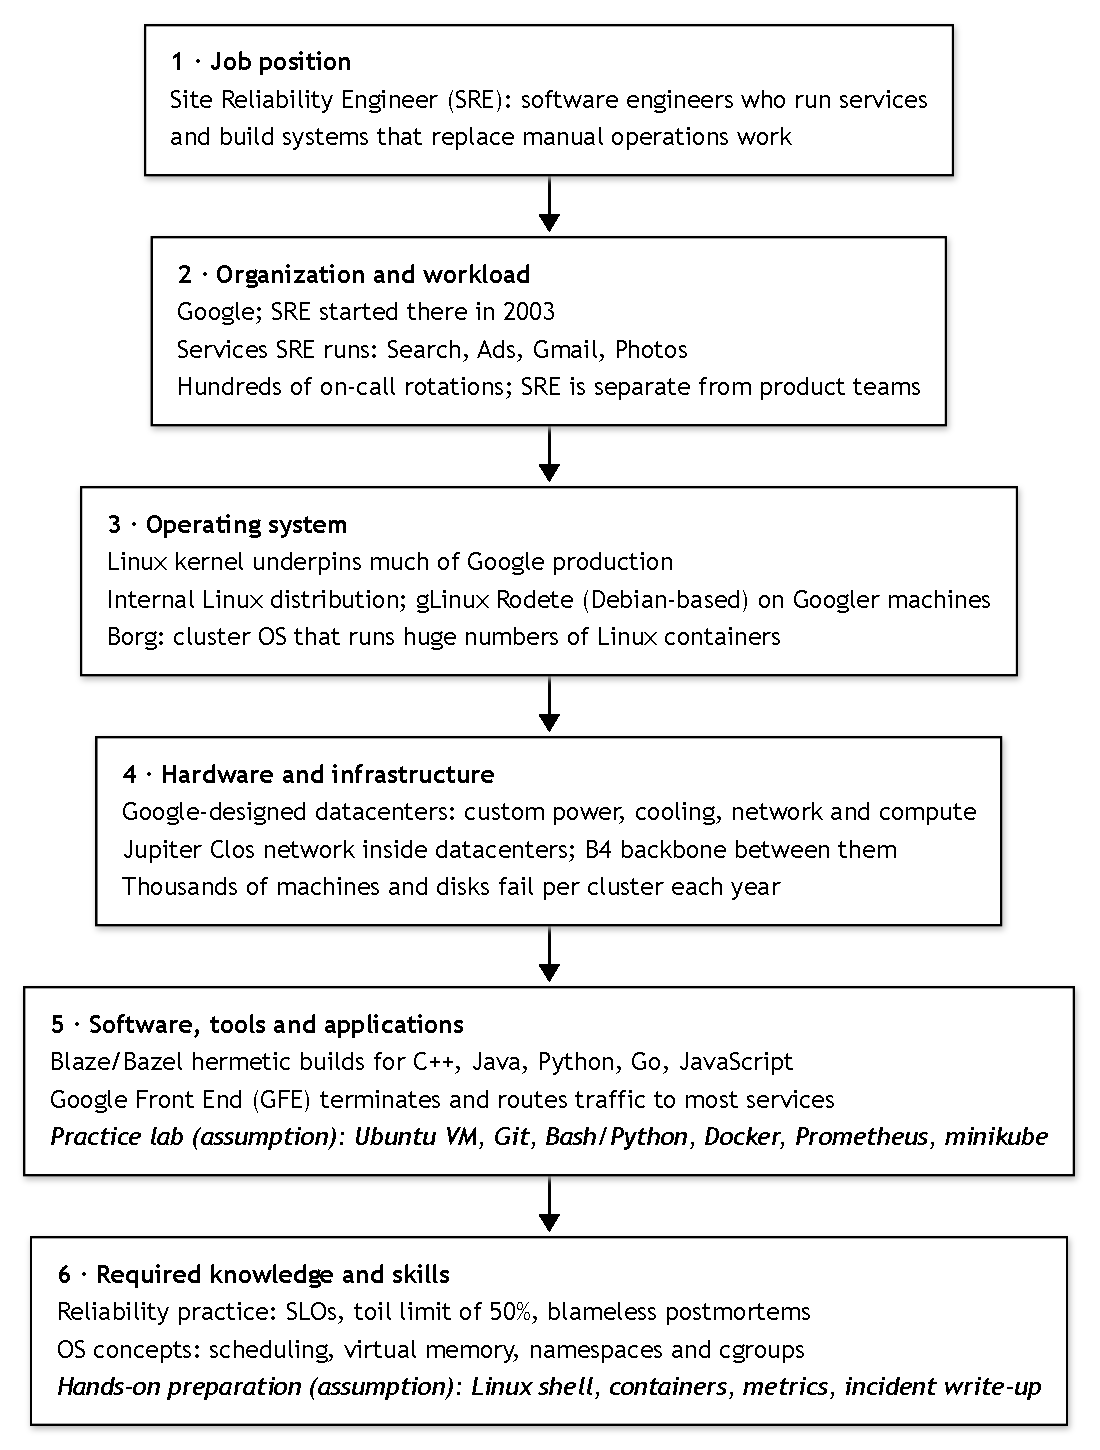
\includegraphics[width=0.94\textwidth,height=0.60\textheight,keepaspectratio]{figures/relationship.pdf}
\caption{From job position to required knowledge and skills for an SRE at Google. Most sources date from 2017 to 2020. Each stage rests on claims from the cited sources \cite{sre-book,workbook,bsrs,google-cloud-blog,static-pdf-incidentmanagementguide-pdf,man7,kernel-docs}. The arrows read: works at, runs on, sits on top of, is operated with, requires. The two italic lines are our assumptions, a typical practice environment and a preparation recommendation, not verified facts about Google. The link from the OS concepts to the job is our interpretation.}
\label{fig:chain}
\end{figure}

\section{Use of Generative AI Platforms/Models}

We used two Generative AI platforms: Claude Code (Anthropic) and Codex (OpenAI). Both are coding agents that we ran in a terminal or desktop session. Table~\ref{tab:genai} lists each platform and model, what we used it for, and how many prompt logs it produced. The complete record is \logsTotal{} prompt logs in the project repository \cite{repo}; \logsSignificant{} of them are marked significant and are reproduced in the Appendix.

\begin{table}[ht]
\centering
% Generated by scripts/make_report_data.py from knowledge-base/ and prompts/. Do not edit by hand.
\begin{tabular}{@{}>{\raggedright\arraybackslash}p{0.34\linewidth}>{\raggedright\arraybackslash}p{0.30\linewidth}r>{\raggedright\arraybackslash}p{0.20\linewidth}@{}}
\hline
Platform and model & Used for & Logs & Period \\
\hline
Claude Code, Claude Opus 5.5 (claude-opus-5-5) & claim research, blind author check, reviewer recheck & 33 & 2026-10-09 to 2026-10-15 \\
Claude Code, Claude Opus 5.5 and Claude Sonnet 5.5 & claim research & 1 & 2026-10-07 \\
Claude Code, Claude Sonnet 5.5 (claude-sonnet-5-5) & claim research, blind author check, reviewer recheck, report drafting & 39 & 2026-10-06 to 2026-10-16 \\
Codex, gpt-6.1-sol & claim research, blind author check & 10 & 2026-10-10 to 2026-10-12 \\
\hline
\end{tabular}

\caption{GenAI platforms and models used, from the prompt logs.}
\label{tab:genai}
\end{table}

\paragraph{How we used GenAI.}
GenAI helped us read and organise sources. It did not decide what is true. Each statement in our knowledge base is a claim with a published source, an access date and an exact sentence copied from that source. A claim passed through four steps:
\begin{enumerate}
  \item \textbf{Research.} An agent read published sources (mainly the Google SRE books and official documentation) and proposed claims with a quote.
  \item \textbf{Blind author check.} A fresh agent received only the claim text and the source address, never the stored quote, and said whether the source supports the claim.
  \item \textbf{Reviewer recheck.} A different team member ran the same blind check in a separate session.
  \item \textbf{Human review.} The reviewer opened every cited source. Only then did the claim become ``human-verified''.
\end{enumerate}
Of \claimsTotal{} claims, \claimsHumanVerified{} are human-verified and \claimsAiChecked{} have passed the AI checks but not yet the human review. The remaining \claimsAssumption{} are assumptions and recommendations. They have no source by design, are labelled as such, and can never become human-verified.

\paragraph{What we corrected.}
The checks changed the content. A reviewer recheck found that the phrase ``not a fixed limit'' went beyond what the SRE book page says, and we replaced the claim with one that stays inside the source. A recheck of 24 claims marked 10 as unreachable because the source site could not be opened, and we rechecked those 10 using archived and mirrored copies. After a review of one pull request, we dropped, reworded and retyped claims about server and database software. Reworded claims went through the blind check again; in one recheck, two of three claims were supported and one only partly.

\paragraph{Report creation.}
We also used GenAI to draft report text and to create the relationship diagram in Figure~\ref{fig:chain}. A team member edited and verified every draft. The prompts for this work are in the Appendix.

\section{Conclusion}\label{sec:conclusion}

Figure~\ref{fig:chain} shows how our findings fit together, from the job position to the knowledge it requires.

\begin{figure}[p]
\centering
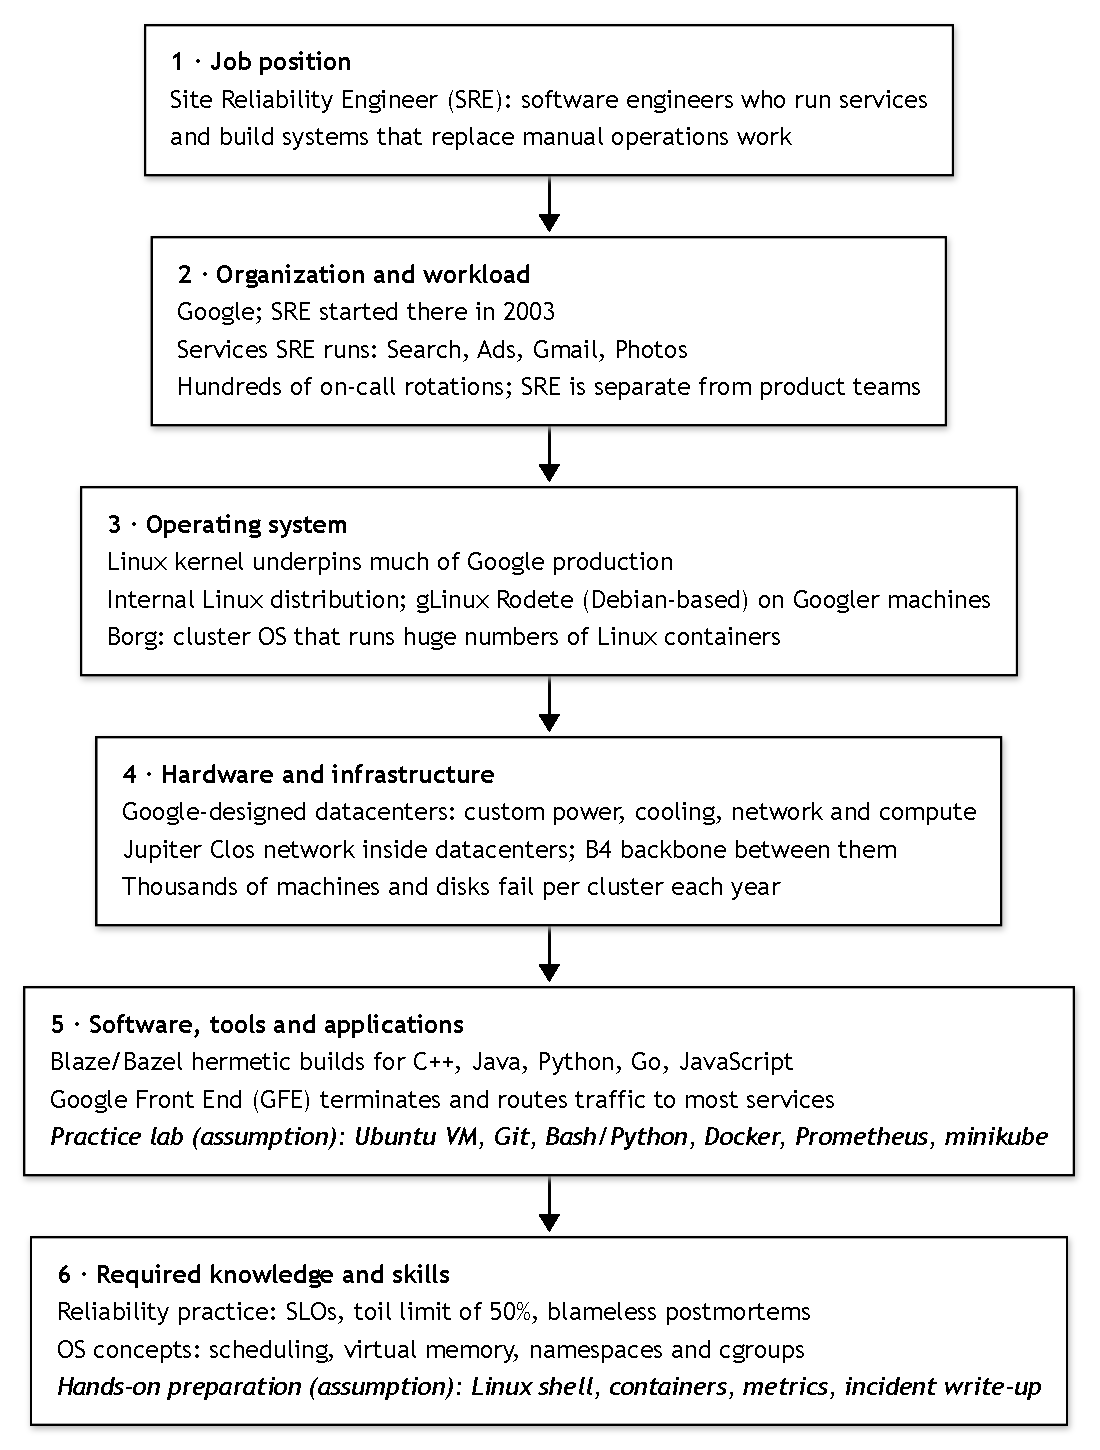
\includegraphics[width=0.94\textwidth,height=0.78\textheight,keepaspectratio]{figures/relationship.pdf}
\caption{From job position to required knowledge and skills for an SRE at Google. Each stage rests on human-verified claims from the cited sources \cite{sre-book,workbook,bsrs,cloud-google-blog-topics-developers-practitioners-how-google-got-to-rolling-linux-releases-for-desktops,static-pdf-incidentmanagementguide-pdf,man7-linux-man-pages-man7-sched-7-html,man7-linux-man-pages-man2-mmap-2-html,man7-linux-man-pages-man7-namespaces-7-html,docs-kernel-admin-guide-cgroup-v2-html}. The arrows read: works at, runs on, sits on top of, is operated with, requires. The two italic lines are our assumptions, a typical practice environment and a preparation recommendation, not verified facts about Google. The link from the OS concepts to the job is our interpretation.}
\label{fig:chain}
\end{figure}

\paragraph{What we found.}
At Google, SRE means software engineers who run services and build systems to replace manual operations work, with operational work limited to 50\% of a team's time \cite{sre-book,workbook}. The work runs on Linux: the kernel underpins much of Google's production infrastructure \cite{bsrs}, and Borg, the cluster operating system, runs huge numbers of Linux containers \cite{sre-book,workbook}. It runs in Google-designed datacenters where thousands of machines and disks fail in a typical year in one cluster \cite{sre-book}. Containers rely on Linux namespaces and control groups and share one kernel \cite{man7-linux-man-pages-man7-namespaces-7-html,docs-kernel-admin-guide-cgroup-v2-html,docs-docker-get-started-docker-concepts-the-basics-what-is-a-container}. In our reading, this links the job to process management, scheduling, virtual memory and resource control, but that link is our interpretation. The SRE book names UNIX system internals and networking (Layer 1 to Layer 3) as the two most common alternate technical skills it seeks \cite{sre-book}.

\paragraph{What we could not find.}
In the sources we read, we found no statement of which operating system Google SREs use on their own workstations. We found no description of an SRE internship program, its eligibility, locations or how to apply. We found no company history, revenue or customer counts beyond the examples in the SRE books, and no list of which CI/CD tools Google SRE uses now. We also found no source on projects given to student SREs. These gaps are noted where they arise. Anything about Google's internal environment that no source states is labelled as an assumption.

\paragraph{Reflection.}
GenAI sped up reading and organising sources, but it made mistakes that human review had to catch. We kept Generative AI output only where a source and a human check supported it.


% Remove the extra space between reference entries to save pages (the font stays 12pt).
\makeatletter
\let\oldthebibliography\thebibliography
\renewcommand\thebibliography[1]{\oldthebibliography{#1}\setlength{\itemsep}{0pt}\setlength{\parsep}{0pt}\sloppy}
\makeatother
\bibliographystyle{unsrt}% classic BibTeX: works in tectonic, TeX Live and Overleaf without biber
\bibliography{references}

\appendix
\section{Complete GenAI Prompts}
\sloppy
These are the complete prompts that we typed to the GenAI platforms in the interactions that produced work we rely on, in order and word for word. \texttt{[REDACTED:kind]} marks a span removed for privacy. A reply of 12 characters or fewer, such as ``yes'', is not shown and is not counted as significant. A turn that gave only a routine instruction, such as to fix a layout detail, find a file, report status or run a git or sign-off step, and shaped no report text, claim or decision, is not shown either. Each prompt is labelled with its turn number in the full log, the count of shown prompts is given in each entry, and the full log holds every turn. The replies and the tool-call records of each session are in the full log named in each entry, in the project repository \cite{repo}.

% Generated by scripts/make_report_data.py from knowledge-base/ and prompts/. Do not edit by hand.

\subsection{Knowledge exploration}

\paragraph{Knowledge exploration 1: Plan and research the topic 04, 05 and 06 claims (OS, hardware, architecture) from the Google SRE books and official Google sources.}
Claude Code (desktop app), Claude Opus 5.5 (claude-opus-5-5); 2026-10-09; log \texttt{2026-10-09-csinside-sre-books-04-06-research}; supporting data: repository file \texttt{docs/\allowbreak{}FinalAssignment\_204341\_1\_69\_AIAssignProject-1.pdf}; 1 web page (sre.google 1). Prompts (5 of 6):
\begin{promptlist}
\item \textbf{Turn~1.} @"[REDACTED:path]" \\{}
\thai{ยังไม่ต้องเขียนอะไร} just plan \thai{สรุปมาอย่างง่ายว่าทำอะไรบ้าง หัวของที่เราได้เน้นทำคือ} \\{}
04-operating-systems \\{}
05-hardware-requirements \\{}
06-system-architecture-infrastructure \\{}
\thai{หัวข้องอื่นจะเป็นของเพื่อน} \\{}
\thai{เอกสารอ้างอิงหลักคือ} https:/\allowbreak{}/\allowbreak{}sre.google/\allowbreak{}books/\allowbreak{} \\{}
\thai{อยากให้หาว่าควรไปเน้นอ่านที่ส่วนไหน วางแผนการจัดสรรเนื้อหา}
\item \textbf{Turn~2.} writing clam 04 05 06 in 2 languages, Thai and English, separate file \\{}
Don't push Thai language file to git hub \\{}
But now don't push anything
\item \textbf{Turn~3.} 04 Are there any points where the information is unclear and requires external research?
\item \textbf{Turn~4.} Have you already looked for the additional information in the documents?
\item \textbf{Turn~5.} Discard the Thai-language files and continue the research; all information used for the write-up must be clear and factually verifiable. \\{}
[Request interrupted by user] \\{}
Discard the Thai-language files and continue the research; all information used for the write-up must be clear and factually verifiable.
\end{promptlist}

\paragraph{Knowledge exploration 2: Research topic 11 OS mechanisms and proposed SRE connections.}
Codex, gpt-6.1-sol; 2026-10-10; log \texttt{2026-10-10-TonCS05-11-os-concepts-research}; supporting data: repository files \texttt{AGENTS.md}, \texttt{docs/\allowbreak{}assignment.md}, \texttt{docs/\allowbreak{}schema.md}, \texttt{knowledge-base/\allowbreak{}11-os-course-concepts/\allowbreak{}index.md}, \texttt{.agents/\allowbreak{}skills/\allowbreak{}research/\allowbreak{}SKILL.md}, \texttt{.agents/\allowbreak{}skills/\allowbreak{}agent-fact-check/\allowbreak{}SKILL.md}; 16 web pages (man7.org 10, docs.kernel.org 2, docs.docker.com 1, kubernetes.io 1, qemu.org 1, sre.google 1). Prompts (1):
\begin{promptlist}
\item \textbf{Turn~1.} \thai{งั้นหาข้อมูลในหัวข้อที่}11\thai{แล้วบันทึกตามกติกาที่ได้ตั้งๆไว้}
\end{promptlist}

\paragraph{Knowledge exploration 3: Research topic 01 (SRE position and job description) into five notes of claims from the Google SRE books and one Google job ad.}
Claude Code (desktop app), Sonnet 5.5 (claude-sonnet-5-5); 2026-10-11; log \texttt{2026-10-11-bximai-01-position-research}; supporting data: 16 web pages (sre.google 15, google.com 1). Prompts (3 of 7):
\begin{promptlist}
\item \textbf{Turn~1.} Main Souce : https:/\allowbreak{}/\allowbreak{}sre.google/\allowbreak{}books/\allowbreak{} \\{}
start research on 01 . Split into 5 notes:

* role-and-duties \\{}
* daily-tasks-and-on-call \\{}
* typical-projects \\{}
* education-and-qualifications \\{}
* environment-overview.

Do one note at a time, starting with role-and-duties

Note : do not made up or guess.
\item \textbf{Turn~2.} Redo 01-06 by the rules: delete its block, re-add it with add\_claim.py using \\{}
the same claim text and quote, then update the claim IDs in Summary and Key points. \\{}
From now on, never hand-edit a claim block. If the wording is wrong, delete and re-add.
\item \textbf{Turn~3.} yes and always follow the instruction rules.
\end{promptlist}

\paragraph{Knowledge exploration 4: Rework the uncommitted 03-soft-skills and 10-server-and-database-software claims and notes to the PR.}
Claude Code, Opus 5.5 (claude-opus-5-5); 2026-10-12; log \texttt{2026-10-12-nine14282-soft-skills-server-db-claims-rework}; supporting data: none. Prompts (2 of 3):
\begin{promptlist}
\item \textbf{Turn~1.} with this standard of writing. Let's look at my old uncommit work 03 and 10 if it need changed, if so, fix those change
\item \textbf{Turn~2.} verify with 2 sub agent again. one for word one for rule
\end{promptlist}

\subsection{Report creation}

\paragraph{Report creation 1: Draft the LaTeX report from the knowledge base, add company and internship claims, build the cover page, and revise the report after a blind review.}
Claude Code (CLI v2.1.299), Claude Sonnet 5.5 (claude-sonnet-5-5); 2026-10-16; log \texttt{2026-10-16-nacs-970-report-drafting-and-review}; supporting data: repository files \texttt{docs/\allowbreak{}assignment.md}, \texttt{docs/\allowbreak{}FinalAssignment\_204341\_1\_69\_AIAssignProject-1.pdf}; 1 web page (google.com 1). Prompts (6 of 35):
\begin{promptlist}
\item \textbf{Turn~1.} list thing that can be add to document assignment
\item \textbf{Turn~2.} 1 i will add it later, we will use latex from now on, i will commit most of work on main now so update workflow \\{}
2 we select sre because we see oppuritunity in ai era that need site engineer since ai still can only do software stuff,  google because big commpany and have delicate website on sre \\{}
3 look in prompt log \\{}
4 draft it for me \\{}
5 mermaid preview it for me first \\{}
6 mermaid \\{}
7 check repo \\{}
8 create it \\{}
-{}-{}- \\{}
recheck un verified topic \\{}
why 13 exisist is it really require by instuctor?
\item \textbf{Turn~14.} i recheck everything it's ok, but recheck for weak/\allowbreak{}example claim
\item \textbf{Turn~22.} 1 group website and book together, and appenddix only really importance log
\item \textbf{Turn~24.} in what we clound not found this is https:/\allowbreak{}/\allowbreak{}www.google.com/\allowbreak{}about/\allowbreak{}careers/\allowbreak{}applications/\allowbreak{} look for internship program, search company history google, search for revenue or customer counts too. don't mention of no human sign off in report
\item \textbf{Turn~35.} start blind agent check of report is it match the instuctor requirement, \\{}
write a review
\end{promptlist}


\end{document}
